\documentclass[a4paper]{article}

\usepackage{tabularx}
\usepackage[portuguese]{babel}
\usepackage[utf8]{inputenc}
\usepackage{indentfirst}
\usepackage{graphicx}
\usepackage{verbatim}
\usepackage{wrapfig}
\usepackage{booktabs}
\usepackage{placeins}
\graphicspath{ {./img/} }

\begin{document}

\setlength{\textwidth}{16cm}
\setlength{\textheight}{22cm}

\title{\Huge\textbf{Adaptoid}\linebreak\linebreak\linebreak
\Large\textbf{Relatório Final}\linebreak\linebreak
\linebreak\linebreak

\includegraphics[scale=0.1]{feup-logo.png}\linebreak\linebreak
\linebreak\linebreak
\Large{Mestrado Integrado em Engenharia Informática e Computação} \linebreak\linebreak
\Large{Programação em Lógica}\linebreak
}

\author{\textbf{Grupo 04 : Adaptoid}\\ David Azevedo - 201405846 \\ João Ferreira - 201404332 \\\linebreak\linebreak \\
 \\ Faculdade de Engenharia da Universidade do Porto \\ Rua Roberto Frias, s\/n, 4200-465 Porto, Portugal \linebreak\linebreak\linebreak
\linebreak\linebreak\vspace{1cm}}
\date{Novembro de 2016}
\maketitle
\thispagestyle{empty}

%************************************************************************************************
%************************************************************************************************

\newpage

\section*{Resumo}
O problema abordado consitiu na implementação do jogo de tabuleiro "Adaptoid" na linguagem Prolog, o que nos representou como sendo um novo desafio, visto que, o grupo não estava familiarizado com este paradigma de programação em lógica. Os objectivos do projecto incluiram : permitir três modos de utilização (Humano/Humano, Humano/Computador, Computador/Computador), incluir dois níveis de jogo para o computador, interface adequada em modo de texto. O trabalho foi elaborado com base em 5 passos fundamentais implementados pela seguinte ordem :
\begin{enumerate}
    \item Representação do tabuleiro em Prolog usando códigos ASCII.
    \item Implementação das regras do jogo em predicados lógicos.
    \item Criação de uma interface simples com o utilizador.
    \item Desenvolvimento de uma pseudo AI para as jogadas do computador.
    \item Design de um sistema simples de menus para completar um ambiente de jogo.
\end{enumerate}
Todos os objectivos foram cumpridos sendo que temos um jogo completo e jogável desenvolvido em Prolog. Desenvolver um jogo funcional numa linguagem nova com a qual apenas se teve contacto durante algumas semana não é fácil, pelo que o grupo no inicio encontrou algumas dificuldades. Após uma leitura extensiva dos slides facultados pelos docentes assim como informação disponível na web foi possível obter uma melhor percepção desta linguagem e paradigma de programação por forma a desenvolver uma aplicação.
Concluindo, ambos os estudantes orgulham-se agora do resultado obtido e do método como tal foi alcançado, podemos também afirmar que o nosso conhecimento de Prolog aumentou consideravelmente.
\newpage

\tableofcontents

%************************************************************************************************
%************************************************************************************************

%*************************************************************************************************
%************************************************************************************************

\newpage

%%%%%%%%%%%%%%%%%%%%%%%%%%
\section{Introdução}

Este projecto foi proposto no âmbito da unidade curricular de Programação em Lógica do Mestrado Integrado de Engenharia Informática e de Computação. Consiste na adaptação de um jogo de tabuleiro para dois jogadores na linguagem Prolog. O tema escolhido foi o "Adaptoid" um jogo relativamente simples de compreender e aprender a jogar, mas que a quantidade de opções disponíveis ao jogador fazem com que o jogo tenha uma complexidade muito superior relativa ao que aparenta.
Este relatório tem a seguinte estrutura :
 \begin{itemize}
   \item Descrição do jogo, a sua história e regras.
   \item Implementação da lógica do jogo em Prolog.
   \item Forma de representação do estado do tabuleiro e sua visualização.
   \item Execução de movimentos.
   \item Verificação do cumprimento das regras do jogo.
   \item Determinação do final do jogo.
   \item Cálculo das jogadas a realizar pelo computador.
   \item Módulo de interface com o utilizador em modo de texto.
   \item Conclucões.
   \item Bibliografia.
   \item Anexos.
 \end{itemize}

\newpage
%%%%%%%%%%%%%%%%%%%%%%%%%%
\section{O Jogo Adaptoid}

\begin{wrapfigure}{r}{0.22\textwidth}
    \centering
    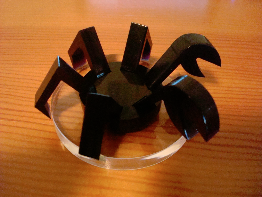
\includegraphics[width=0.22\textwidth]{adaptoid}
    \caption{Imagem ilustratica de um "adaptoid"}
\end{wrapfigure}

Adaptoid é um jogo de tabuleiro para dois jogadores, constituído por um tabuleiro hexagonal, que contém (37 espaços), e por um conjunto de criaturas denominadas de “adaptoid”. Cabe a cada jogador evoluir o seu “adaptoid” adicionando membros, garras e pernas, ao corpo do adaptoid. Os membros são fatores decisivos, pois fazem variar o comportamento do “adaptoid”. As garras definem o dano e as pernas a capacidade de movimento.

\begin{wrapfigure}{l}{0.20\textwidth}
    	\centering
	\vspace{-10pt}
   	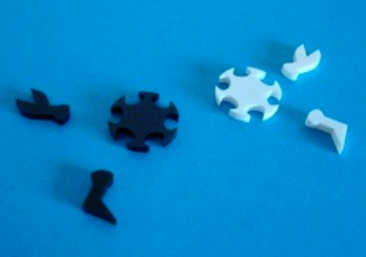
\includegraphics[width=0.20\textwidth]{adaptoidsDissecados}
    	\caption{Corpo e membros de um "adaptoid"}
\end{wrapfigure}

Cada turno divide-se em 3 fases distintas, sendo elas, movimento, crescimento e alimentação. Durante a fase de movimento o jogador pode mover um dos seus “adaptoids”, o número de espaços percorridos depende do número de pernas desse “adaptoid”.

Não é possível mover o adaptoid através de espaços que estejam ocupados, apenas é possível mover em direção a espaços vazios sem obstáculos e mover para o topo de um “adaptoid” oposto, para iniciar a captura. Na fase de crescimento o jogador pode optar por um de dois casos possíveis, ou cria um novo corpo adjacente a um dos seus “adaptoids” existentes, ou então adiciona uma perna, ou garra, a um dos seus “adaptoids” existentes no tabuleiro. Na fase de alimentação, é verificada em cada peça do inimigo se ela está com fome, ou seja, o número  de espaços vazios à sua volta terá que ser igual ou maior ao número de membros do “adaptoid”. No caso de fome, a peça inimiga morre, é removida e é atribuído um ponto ao jogador. Durante a captura o “adaptoid ”com mais garras ganha e o “adaptoid ” derrotado é removido do tabuleiro. Em caso do número de garras dos “adaptoids” ser igual, ambos são removidos e cada jogador recebe um ponto. As peças de “adaptoids” mortos poderão ser novamente usadas. O jogo termina quando um jogador chega aos 5 pontos ou quando um dos jogadores ficar sem nenhum “adaptoid” no tabuleiro.


\begin{figure}[h]
    \begin{center}
        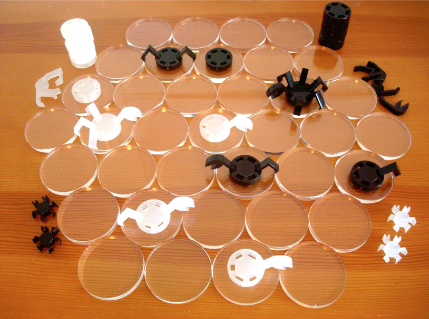
\includegraphics[scale=0.5]{jogoDecorrer}
        \caption{Estado de um jogo de adaptoid}
        \centering
    \end{center}
\end{figure}

\newpage
%%%%%%%%%%%%%%%%%%%%%%%%%%
\section{Lógica do Jogo}

\subsection{Representação do Estado do Jogo}  Para representar o tabuleiro do jogo optámos por uma lista de listas, onde cada uma das listas define uma das linhas do tabuleiro e por consequência cada elemento dessa lista representa uma célula no nosso jogo,  para facilitar a pesquisa de casas adjacentes foi inserido no início de cada lista alguns átomos que mais tarde serão interpretados como espaços por forma a garantir a forma hexagonal definida pelos criadores do jogo. As peças do jogo, os “adaptoids”, são representados usando uma lista de 4 elementos ([Id,Cor,NPernas,NGarras]). Os ID têm como função facilitar na pesquisa das peças no tabuleiro. A Cor assume o valor ‘O’(white) ou ‘X’(black), e representa o jogador ao qual a peça pertence, uma vez que na consola do sicstus não é possível alterar a cor. O NPernas como o nome indica é o número de pernas que a peça possui, idem para o NGarras. Nota: Os átomos ‘a’,’b’,’c’,'d','e','f','g' e ‘\#’ são usados para controlar a posição das casas do jogo relativa à lista que representa a linha do tabuleiro onde estas se encontram, ou seja, com a introdução destes símbolos é possível seguir a seguinte lógica: Para uma determinada célula na posição (x,y), a célula-vizinha imediatamente abaixo do lado esquerdo está na posição (x,y+1) e a célula imediatamente abaixo do lado direito está na posição (x+1,y+1). Neste pequeno exemplo, o jogador da equipa ‘X’(white) ganhou porque o jogador da equipa ‘O’(black) não possui mais nenhuma peça no tabuleiro. Também é possível ambos os jogadores terem peças no tabuleiro e um ganhar, mas neste caso o jogador vencedor alcançou primeiro os 5 pontos.

\subsection{Visualização do Tabuleiro} Originalmente as células do tabuleiro são redondas, mas para efeitos de visualização utilizando caracteres ASCII, estas são representadas como hexágonos. Com este formato, para ser possível o desenho do “adaptoid” contendo as suas garras e pernas seguiu-se a seguinte estratégia: Nesta célula é possível observar todas as posições possíveis para as garras(símbolo Y ) e pernas(símbolo L), este caso é impossível já que o número máximo de membros é 6, mas para efeitos de demonstração do funcionamento, é possível observar que as garras(Y) são desenhadas apenas no topo e no meio (caso sejam 6 garras no total), o mesmo acontece para as pernas. O símbolo B representa a cor do “adaptoid” e à sua volta está o número dessa peça.
Para que o desenho de cada célula seja possível, para cada linha do conteúdo do tabuleiro são desenhadas 4 linhas no ecrã, sendo elas:

\begin{table}[h!]
  \centering
  \caption{Legenda das camadas de uma célula.}
  \label{tab:table1}
 \newcolumntype{P}[1]{>{\centering\arraybackslash}p{#1}}
  \begin{tabular}{ c |  P{9.8cm}}
	\hline &
	\\
	
\includegraphics[width=0.1\textwidth]{topo}
           & A linha de topo que contém o número de garras (até 5 garras).
	\\&
	\\
	
	
\includegraphics[width=0.1\textwidth]{meio}
	& A linha do meio que contém o sexto membro (garra/perna), a cor e  número da peça.
	\\

	
\includegraphics[width=0.1\textwidth]{baixo}
	& A linha de baixo que contém o número de pernas (até 5 pernas).

	\\
	
\includegraphics[width=0.06\textwidth]{separacao}
	& A linha de separação para ser possível uma melhor distinção entre células adjacentes.
	\end{tabular}
\end{table}
\FloatBarrier
Foram utilizados símbolos especiais que apenas são usados como espaçamento, para que seja possível enquadrar as células no seu local. O predicado de visualização já se encontra 100\% desenvolvido sendo que recebe um tabuleiro no formato de lista de listas e procede ao desenho no mesmo na consola como se pode ver na figura ao lado.

\subsection{Lista de Jogadas Válidas}Foram implementados predicados que definem as jogadas válidas, estes predicados implementam as jogadas propriamente ditas e validam no caso do utilizador, no caso do computador são usados para obter a lista de jogadas possíveis. As três regras que se seguem dizem respeito às diferentes fases de que cada jogada (Movimento(M), Evolução(E) e Alimentação(famintos)).
\begin{itemize}
    \item \textit{lerRegraM(+Cor,+Acao,+JogoInicial,-JogoFinal)} , as ações possíveis incluem \textit{mover(+X,+Y,+Ori)} e \textit{capturar(+X,+Y,+Ori)}.
    \item \textit{lerRegraE(+Cor,+Acao,+JogoInicial,-JogoFinal)} , as ações incluem \textit{aP(+X,+Y)} para adicionar uma perna, \textit{aG(+X,+Y)} para adicionar uma garra e \textit{aC(+X,+Y,+Ori)} para adicionar um novo adaptoid.
    \item \textit{famintos(+JogoInicial,+Cor,-JogoFinal)}.
\end{itemize}

\subsection{Execução de Jogadas} Validação e execução de uma jogada num tabuleiro, obtendo o novo estado do jogo. Exemplo: \textit{move(+Move, +Board, -NewBoard)}.
\begin{itemize}
    \item \textit{capturar(+JogoInicial, +ID, +Cor, +Ori, -JogoFinal)}.
    \item \textit{moverPeca(+JogoInicial, +ID, +Cor, +Ori, -JogoFinal)}.
    \item \textit{addPerna(+Board, +Cor, +ID, -NewBoard)}.
    \item \textit{addGarra(+Board, +Cor, +ID, -NewBoard)}.
    \item \textit{esfomeados(+OriginalBoard, +BoardCopy, +Cor, -Nremovidos, -NewBoard)} esta função não é usada diretamente pelo utilizador mas é feita no final de cada jogada.
    \item \textit{addCorpo(+Board, +ID, +Cor, +Ori, -NewBoard)}.
\end{itemize}

\subsection{Avaliação do Tabuleiro} Avaliação do estado do jogo, que permitirá comparar a aplicação das diversas jogadas disponíveis. Exemplo: \textit{value(+Board, +Player, -Value)}.

\subsection{Final do Jogo} Verificação do fim do jogo, com identificação do vencedor. \\Exemplo: \textit{game\_over(+Board, -Winner)}.

\subsection{Jogada do Computador} Escolha da jogada a efetuar pelo computador, dependendo do nível de dificuldade. Por exemplo: \textit{choose\_move(+Level, +Board, -Move)}.


%%%%%%%%%%%%%%%%%%%%%%%%%%
\section{Interface com o Utilizador}

Descrever o módulo de interface com o utilizador em modo de texto.


%%%%%%%%%%%%%%%%%%%%%%%%%%
\section{Conclusões}
Que conclui deste projecto? Como poderia melhorar o trabalho desenvolvido?


\clearpage
%\addcontentsline{toc}{section}{Bibliografia}
%\renewcommand\refname{Bibliografia}
%\bibliographystyle{plain}
%\bibliography{myrefs}

\newpage
\appendix
\section{Nome do Anexo}
Código Prolog implementado devidamente comentado e outros elementos úteis que não sejam essenciais ao relatório.

\end{document}
